%\documentclass[trans]{beamer}
\documentclass[10pt]{beamer}

% Try the class options [notes], [notes=only], [trans], [handout],
% [red], [compress], [draft], [class=article] and see what happens!

% Copyright 2003 by Till Tantau <tantau@users.sourceforge.net>.
%
% This program can be redistributed and/or modified under the terms
% of the LaTeX Project Public License Distributed from CTAN
% archives in directory macros/latex/base/lppl.txt.

% For a green structure color use:
%\colorlet{structure}{green!50!black}

%%%%%%%%%% User macros%%%%%%%%%%%
\newcommand{\mypurple}[1]{{\color[rgb]{0.7,0,0.8}#1}}
\newcommand{\myred}  [1] {{\color{red}#1}}
\newcommand{\myblue} [1] {{\color{blue}#1}}
\newcommand{\mygreen}[1] {{\color[rgb]{0,0.5,0}#1}}
\newcommand{\Nat}{\mathbb{N}}
\def\sla  {\!\!\!\slash}
%%%%%%%%%%%%%%%%%%%%%%%%%%%%%%%%%
\mode<article> % only for the article version
{
  \usepackage{beamerbasearticle}
  \usepackage{fullpage}
  \usepackage{hyperref}
}

%\beamertemplateshadingbackground{red!10}{blue!10}
%\beamertemplateshadingbackground{blue!10}{blue!10}

%\usepackage{beamerthemeshadow}

\usepackage{pgf,pgfarrows,pgfnodes,pgfautomata,pgfheaps,pgfshade}
\usepackage{amsmath,amssymb}
\usepackage[latin1]{inputenc}
\usepackage{colortbl}
\usepackage[english]{babel}
%\usepackage{verbatim}
%\usepackage{listings}
\usepackage[procnames]{listings}

%\usepackage{lmodern}
\usepackage[T1]{fontenc} 

\usepackage{times}

% for code colouring
\include{pythonlisting}
\include{cpplisting}

% Use some nice templates
\beamertemplatetransparentcovereddynamic
\usetheme{Binet}
%\usetheme{Madrid}
%\usetheme{Boadilla}
%\usetheme{Berkeley}
%\usetheme{Rochester}

%\def\command#1{\list{}{\leftmargin=2em\itemindent-\leftmargin\def\makelabel##1{\hss##1}}%
%\item\extractcommand#1@\par\topsep=0pt}
%\def\endcommand{\endlist}
%\def\extractcommand#1#2@{\strut\declare{\texttt{\string#1}}#2}

%
% The following info should normally be given in you main file:
%

\hypersetup{%
  pdftitle={AthenaMT/AthenaMP},%
  pdfauthor={Sebastien Binet},
  pdfsubject={AthenaMP},
  pdfkeywords={ATLAS,Athena,python,COW,parallelization},
%  pdfpagemode=FullScreen%
}

\title[AthenaMT/AthenaMP]{Harnessing multicores:\\ strategies and implementations in \textsc{Atlas}}
\author[S. Binet]{S\'ebastien~Binet,\\ Paolo~Calafiura, Scott~Snyder,\\ Werner~Wiedenmann, Frank~Winklmeier}%\inst{1}
%% \institute[LBL]{
%% %  \inst{1}%
%%   Lawrence Berkeley Laboratory}
\date{24-03-2009 CHEP09}

%% \begin{center}
%%  On behalf of many people:\\
%%  Paolo Calafiura, Scott Snyder,\\
%%  Werner Wiedenmann, Frank Winklmeier
%% \end{center}

\pgfdeclaremask{atlaslogo}{atlaslogo}
%\pgfdeclaremask{ubp}{UBP-logo}
\pgfdeclareimage[mask=atlaslogo,width=2cm]{atlas-logo}{atlaslogo}
%\pgfdeclareimage[mask=ubp,width=1cm]{ubp-logo}{UBP-logo}

\logo{%
  \vbox{%
    \hfil\pgfuseimage{atlas-logo}%
    %\hbox to 1cm{\hfil\pgfuseimage{atlas-logo}}%
    %\vskip0.1cm%
    %\hbox{\pgfuseimage{ubp-logo}}%
  }%
}


\begin{document}
\lstset{language=C++}

\frame{\titlepage
%  \hskip0.44\paperwidth
%  \insertlogo

    \begin{beamercolorbox}[sep=8pt,center,fg]{mylogo}
      \usebeamercolor[fg]{mylogo}\insertlogo
    \end{beamercolorbox}

}

%\section*{Outline}
%\frame{\tableofcontents[part=1]}%,pausesections]}

%\AtBeginSubsection[]
%{
%  \frame<handout:0>
%  {
%    \frametitle{Outline}
%    \tableofcontents[current,currentsubsection]
%  }
%}

\part<presentation>{Main Talk}

%%%%%%%%%%%%%%%%%%%%%%%%%%%%%%%%%%%%%%%%%%%%%%%%%%%%%%%%%%%%%%%%%%%%%%%%%%%%%%%
%%%%%%%%%%%%%%%%%%%%%%%%%%%%%%%%%%%%%%%%%%%%%%%%%%%%%%%%%%%%%%%%%%%%%%%%%%%%%%%
%\section[Outline]{Outline}

% \frame<beamer>{
%   \frametitle{Outline}
%   \begin{columns}
% \begin{column}{0.49\textwidth}
%   \begin{block}{}
%   \tableofcontents
%   \end{block}
% \end{column}
% \end{columns}

% }
%\frame{\partpage}

%%%%%%%%%%%%%%%%%%%%%%%%%%%%%%%%%%%%%%%%%%%%%%%%%%%%%%%%%%%%%%%%%%%%%%%%%%%%%%%
%%%%%%%%%%%%%%%%%%%%%%%%%%%%%%%%%%%%%%%%%%%%%%%%%%%%%%%%%%%%%%%%%%%%%%%%%%%%%%%
\section[Outline]{Outline}

\frame{
  \frametitle{Outline}

  \begin{columns}
    \begin{column}{0.8\textwidth}
      \begin{block}{}
        \begin{itemize}
          \item Introduction
          \item Experience w/ multi-threading: \texttt{AthenaMT}
          \item Experience w/ multi-processes: \texttt{AthenaMP}
          \item Conclusions
            \begin{itemize}
              \item future plans
            \end{itemize}
        \end{itemize}
      \end{block}
    \end{column}
  \end{columns}
}

%%%%%%%%%%%%%%%%%%%%%%%%%%%%%%%%%%%%%%%%%%%%%%%%%%%%%%%%%%%%%%%%%%%%%%%%%%%%%%%
\section[Introduction]{Introduction}

\frame{
  \frametitle{Introduction}

  \begin{columns}
    \begin{column}{0.8\textwidth}
      \begin{block}{Motivations: hardware trends}
        \begin{itemize}
          \item \emph{CPU} $\Rightarrow$ multicores
          \item large number of \emph{CPU} cores calls for more parallelism
            \begin{itemize}
              \item event parallelism inherent to typical \emph{HEP} selection and reconstruction programs
              \item parallelization inside applications may provide huge speed ups but requires typically also careful (re)design of code
            \end{itemize}
          \item exploit parallelism with:
            \begin{itemize}
              \item multi-threading (\texttt{AthenaMT})
              \item multi-processes (\texttt{AthenaMP})
            \end{itemize}
        \end{itemize}
      \end{block}
    \end{column}
  \end{columns}

}

\frame{
  \frametitle{Introduction - II}

  \begin{columns}
    \begin{column}{0.8\textwidth}
      \begin{block}{Boundary conditions}
        \begin{itemize}
          \item \textsc{Atlas} has large code basis mostly written and designed in \emph{``pre-multi-core era''}
            \begin{itemize}
              \item \emph{online} and \emph{offline} reconstruction code mainly process based and single threaded
            \end{itemize}
          \item experimented with multi-threading and multi-processes:
            \begin{itemize}
              \item existing code basis implies boundary conditions for future developments
              \item modifications have to be as transparent as possible
            \end{itemize}
        \end{itemize}
      \end{block}
    \end{column}
  \end{columns}

}

%%%%%%%%%%%%%%%%%%%%%%%%%%%%%%%%%%%%%%%%%%%%%%%%%%%%%%%%%%%%%%%%%%%%%%%%%%%%%%%
\section[AthenaMT]{AthenaMT}

\frame{
  \frametitle{Multi-threading: \texttt{AthenaMT}}

  \begin{columns}
    \begin{column}{0.9\textwidth}
      \begin{block}{}
        \begin{itemize}
          \item Code sharing
          \item Small context switch times $\rightarrow$ \emph{``lightweight processes''}
          \item Automatic sharing of many hardware resources
          \item Example: Trigger L2 Processing Unit
        \end{itemize}
      \end{block}
    \end{column}
  \end{columns}

  \begin{columns}
    \begin{column}{0.7\textwidth}
      \begin{exampleblock}{}
        \begin{itemize}
        \item Event processing in multiple worker threads
        \item HLT selection software controlled by TDAQ framework
        \item Special version of \texttt{Gaudi/Athena} framework to create selection algorithm instances for worker threads
        \item Development and \emph{MT} tests started on dual processor single core machines, long before multi-core machines were available
        \end{itemize}
        \end{exampleblock}
    \end{column}

    \begin{column}{0.3\textwidth}
      \begin{figure}
        \begin{center}
          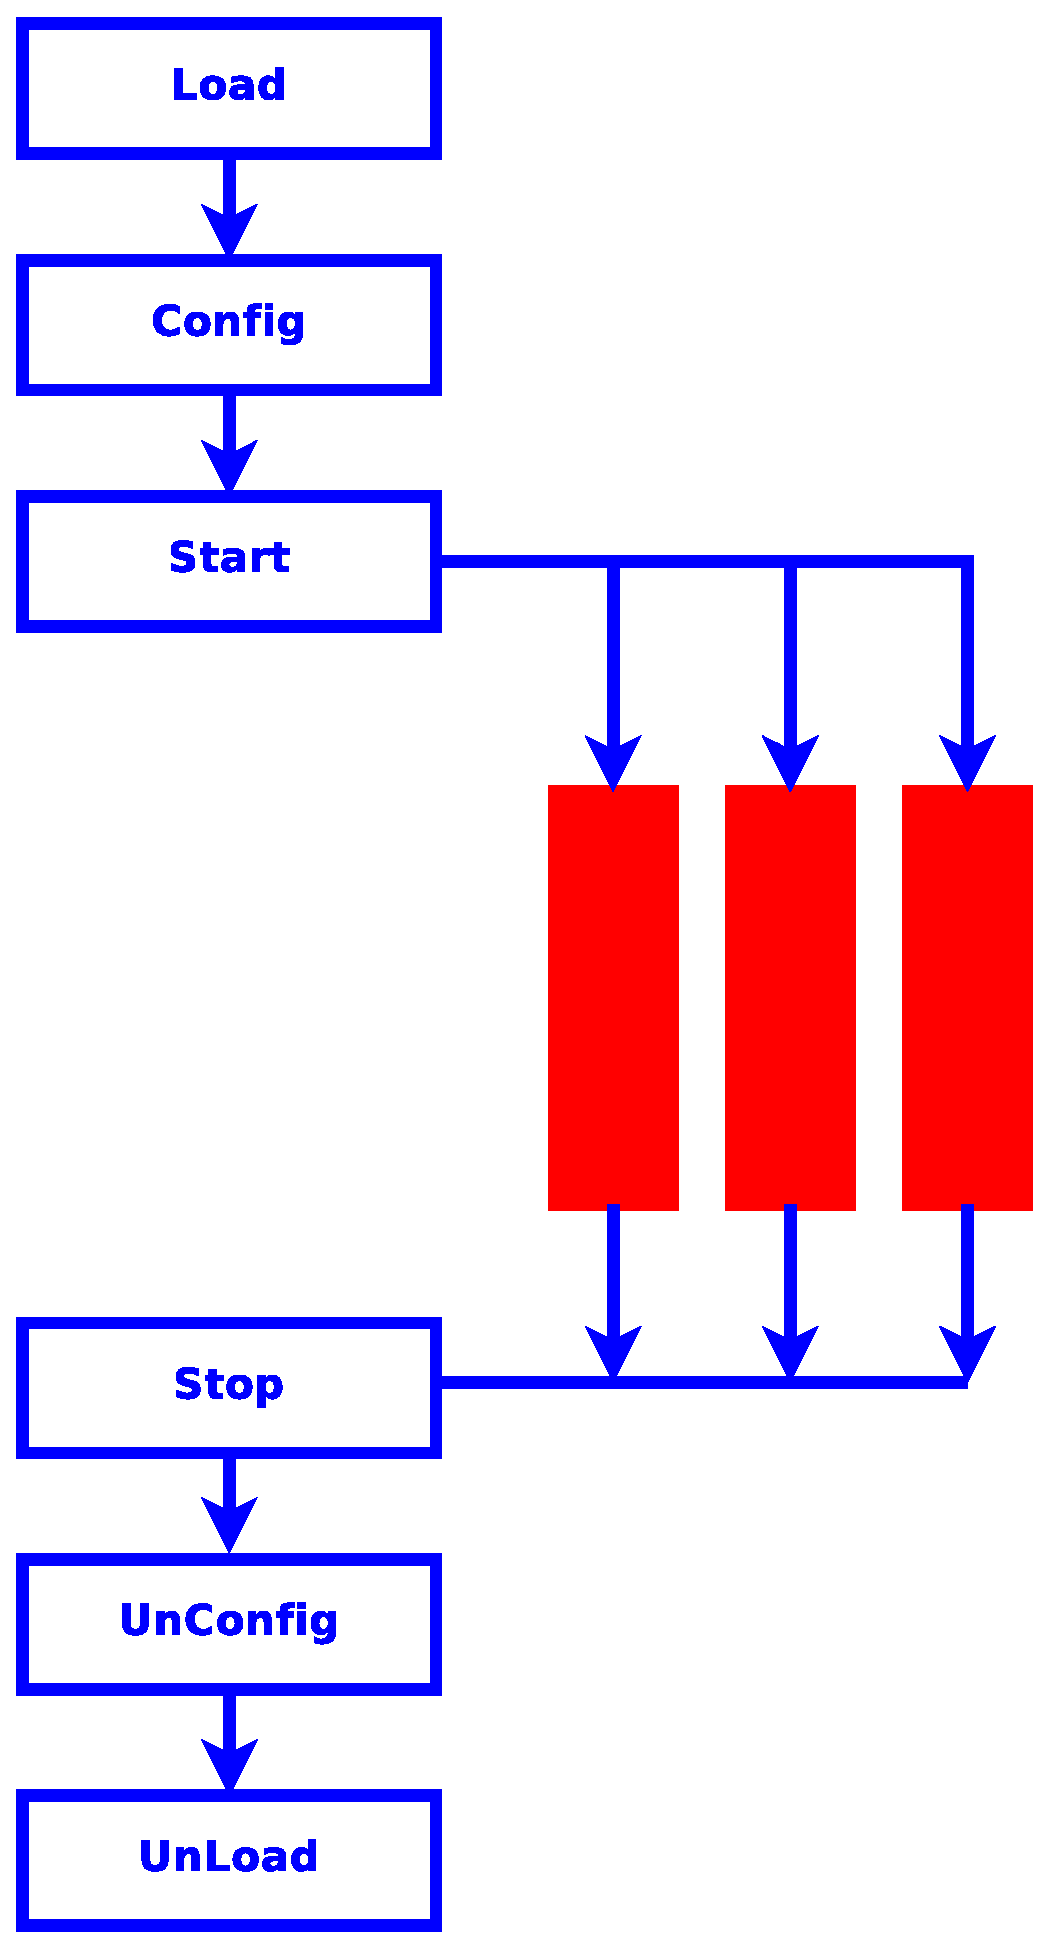
\includegraphics[angle=0,width=0.8\textwidth]{figs/tdaq-mt-flow.eps}
        \end{center}
      \end{figure}
    \end{column}
  \end{columns}
}

\frame{
  \frametitle{Multi-threading support in \texttt{Athena} framework}

%  \begin{columns}
%    \begin{column}{0.9\textwidth}
%      \begin{block}{}
        \begin{itemize}
          \item \myred{Multi-threading:} all services and algorithms which modify data have to be thread specific (\emph{e.g.} \texttt{StoreGate/EventStore})
            \begin{itemize}
              \item threads may however also use \mypurple{``read only''} services which are common to all threads (\emph{e.g.} \texttt{GeometrySvc, DetectorStore})
            \end{itemize}
          \item all thread-specific instances of services and algorithms are distinguished by \myred{type} and \myred{\texttt{(generic name)\_\_(thread ID)}}
            \begin{itemize}
              \item \emph{e.g.} create an algorithm of type \mygreen{\texttt{TriggerSteering}} and generic name \mygreen{\texttt{TrigStr}} for 2 threads:
                \begin{itemize}
                  \item \mygreen{\texttt{TriggerSteering/TrigStr\_\_0}}
                  \item \mygreen{\texttt{TriggerSteering/TrigStr\_\_1}}
                \end{itemize}
            \end{itemize}
          \item Assumption:
            \begin{itemize}
              \item \myred{Algorithms} are \mypurple{always thread specific}
                \begin{itemize}
                  \item for each thread an algorithm copy is generated automatically
                \end{itemize}
              \item if a \myred{Service} is run thread specific or common for all threads has to be specified in the configuration
            \end{itemize}
          \item modified \texttt{Athena} can also be used for normal offline running
        \end{itemize}
%      \end{block}
%    \end{column}
%  \end{columns}

}

\frame{
\frametitle{Experiences with multi-threading}
\begin{block}{}
  \begin{itemize}
    \item created different event selection slices which could run multithreaded
    \item some technical issues are historical now but interesting:
      \begin{itemize}
        \item implementation of \texttt{STL} elements with different compiler versions
          \begin{itemize}
            \item memory allocation model not optimal for \emph{``event parallelism''}
          \end{itemize}
        \item thread safe external libraries
      \end{itemize}
  \end{itemize}
\end{block}

}

\frame{
\frametitle{Experiences with multi-threading - II}
\begin{exampleblock}{Software development}
  \begin{itemize}
    \item developers have to be familiar with thread programming
      \begin{itemize}
        \item need special training and knowledge
      \end{itemize}
    \item developers have to take into account for their code the MT model of L2 $\Rightarrow$ \mypurple{event parallelism}
      \begin{itemize}
        \item created emulator \emph{athenaMT} as a development tool/environment for Lvl2 code
      \end{itemize}
    \item synchronization problems for multi-threaded code are tedious to debug
    \item need good tools to assist developers for debugging and optimizing multi-threaded programs
    \item typically selection code \mypurple{changes rapidly} due to physics needs
      \begin{itemize}
        \item \myred{constant need for re-optimization}
      \end{itemize}
  \end{itemize}
\end{exampleblock}

\begin{alertblock}{}
  \begin{itemize}
    \item \myred{Problem:} preserve thread safe and optimized code over release cycles and in a large heterogeneous developer community
      \begin{itemize}
        \item coupling of different sw communities with different goals
      \end{itemize}
  \end{itemize}
\end{alertblock}
\small{
Presently we run $n$ ($= \# cores$) instances of L2  Processing Unit on a multi-core machine with one worker thread}
}

%%%%%%%%%%%%%%%%%%%%%%%%%%%%%%%%%%%%%%%%%%%%%%%%%%%%%%%%%%%%%%%%%%%%%%%%%%%%%%%
\section[AthenaMP]{AthenaMP}

\frame{
  \frametitle{\texttt{Process-based parallelism}}

  \begin{columns}
    \begin{column}{0.9\textwidth}
      \begin{exampleblock}{}
        \begin{itemize}
          \item run $n$ process instances on machine with $n$ cores
            \begin{itemize}
              \item easy to do with existing code
              \item \emph{a priori} no code changes required
              \item observe good scaling with number of cores
            \end{itemize}
        \end{itemize}
      \end{exampleblock}

      \begin{block}{Problem(s)}
        \begin{itemize}
          \item resource sharing and optimization
          \item resource requirements are multiplied w/ nbr of process instances
          \item \myred{memory size}
          \item OS resources: file descriptors, network sockets, \ldots
          \item on trigger farms:
            \begin{itemize}
              \item number of controlled applications
              \item number of network connections to readout system
              \item transfer of same configuration data $n$ times to the same machine
              \item recalculation of the same configuration data $n$ times
              \item optimal \emph{CPU} utilization: use \emph{CPU} for event processing while waiting for input data
            \end{itemize}
        \end{itemize}
      \end{block}

    \end{column}
  \end{columns}
}

\frame{
  \frametitle{Memory sharing via \texttt{fork}}
  \begin{itemize}
    \item Basic idea:
      \begin{itemize}
        \item run multiple \texttt{Athena} reconstruction jobs, sharing as much memory as possible
        \item minimize number of required code changes
          \begin{itemize}
            \item let the OS do most of the work
          \end{itemize}
        \item use {\bf\myred{\texttt{fork()}}}
      \end{itemize}
    \item \texttt{fork()}:
      \begin{itemize}
        \item \texttt{fork()} clones a process, including its entire address space
        \item modern OS' \texttt{fork()} uses \mypurple{\emph{``Copy On Write''}}
          \begin{itemize}
            \item memory is shared up to the point a process writes to it
            \item memory will be copied and the affected changes will become unshared
          \end{itemize}
        \item \texttt{fork()} as late as possible but before any output is written
        \item as much memory as possible is \mypurple{automatically shared} between processes
          \begin{itemize}
            \item memory which is modified will become unshared
            \item static configuration data will remain shared
          \end{itemize}
      \end{itemize}
  \end{itemize}
}

\frame{
  \frametitle{Memory sharing via \texttt{fork} - II}
\begin{block}{}
\begin{itemize}
  \item advantages:
    \begin{itemize}
      \item \mypurple{all} memory that can be shared \mypurple{will be}
      \item code changes restricted to few framework packages, bulk of the code remains untouched
      \item don't need to worry about \mygreen{locking}
    \end{itemize}
\end{itemize}
\end{block}

\begin{exampleblock}{}
  \begin{itemize}
    \item disadvantages
      \begin{itemize}
        \item memory can not be \mypurple{re-shared} after it became unshared
          \begin{itemize}
            \item maybe a problem for conditions data
          \end{itemize}
      \end{itemize}
  \end{itemize}
\end{exampleblock}

\begin{figure}
  \begin{center}
    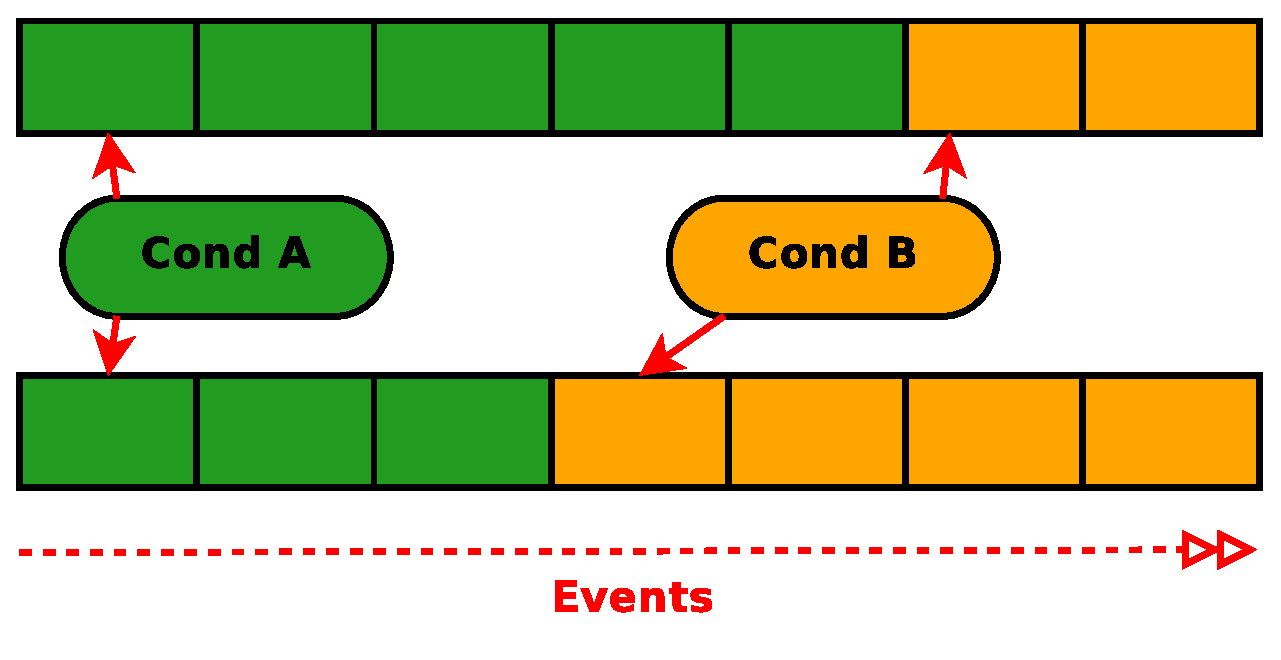
\includegraphics[angle=0,width=0.65\textwidth]{figs/cond-data-flow.eps}
  \end{center}
\end{figure}
}

\frame{
  \frametitle{\texttt{AthenaMP} implementation}

  \begin{columns}
    \begin{column}{0.95\textwidth}

      \begin{block}{}
        \begin{itemize}
          \item avoid clients' changes
          \item hide MP-semantics \myred{inside} \texttt{Athena} instead of publishing them as a layer on top
          \item use the \texttt{python} module \mygreen{\texttt{multiprocessing}} (backported from 2.6) for the process management
          \item write a new event loop manager as a usual \texttt{Gaudi} component to encapsulate the parallelism handling
          \item modify the I/O-related components appropriately
        \end{itemize}
      \end{block}

    \end{column}
  \end{columns}

\begin{figure}
  \begin{center}
    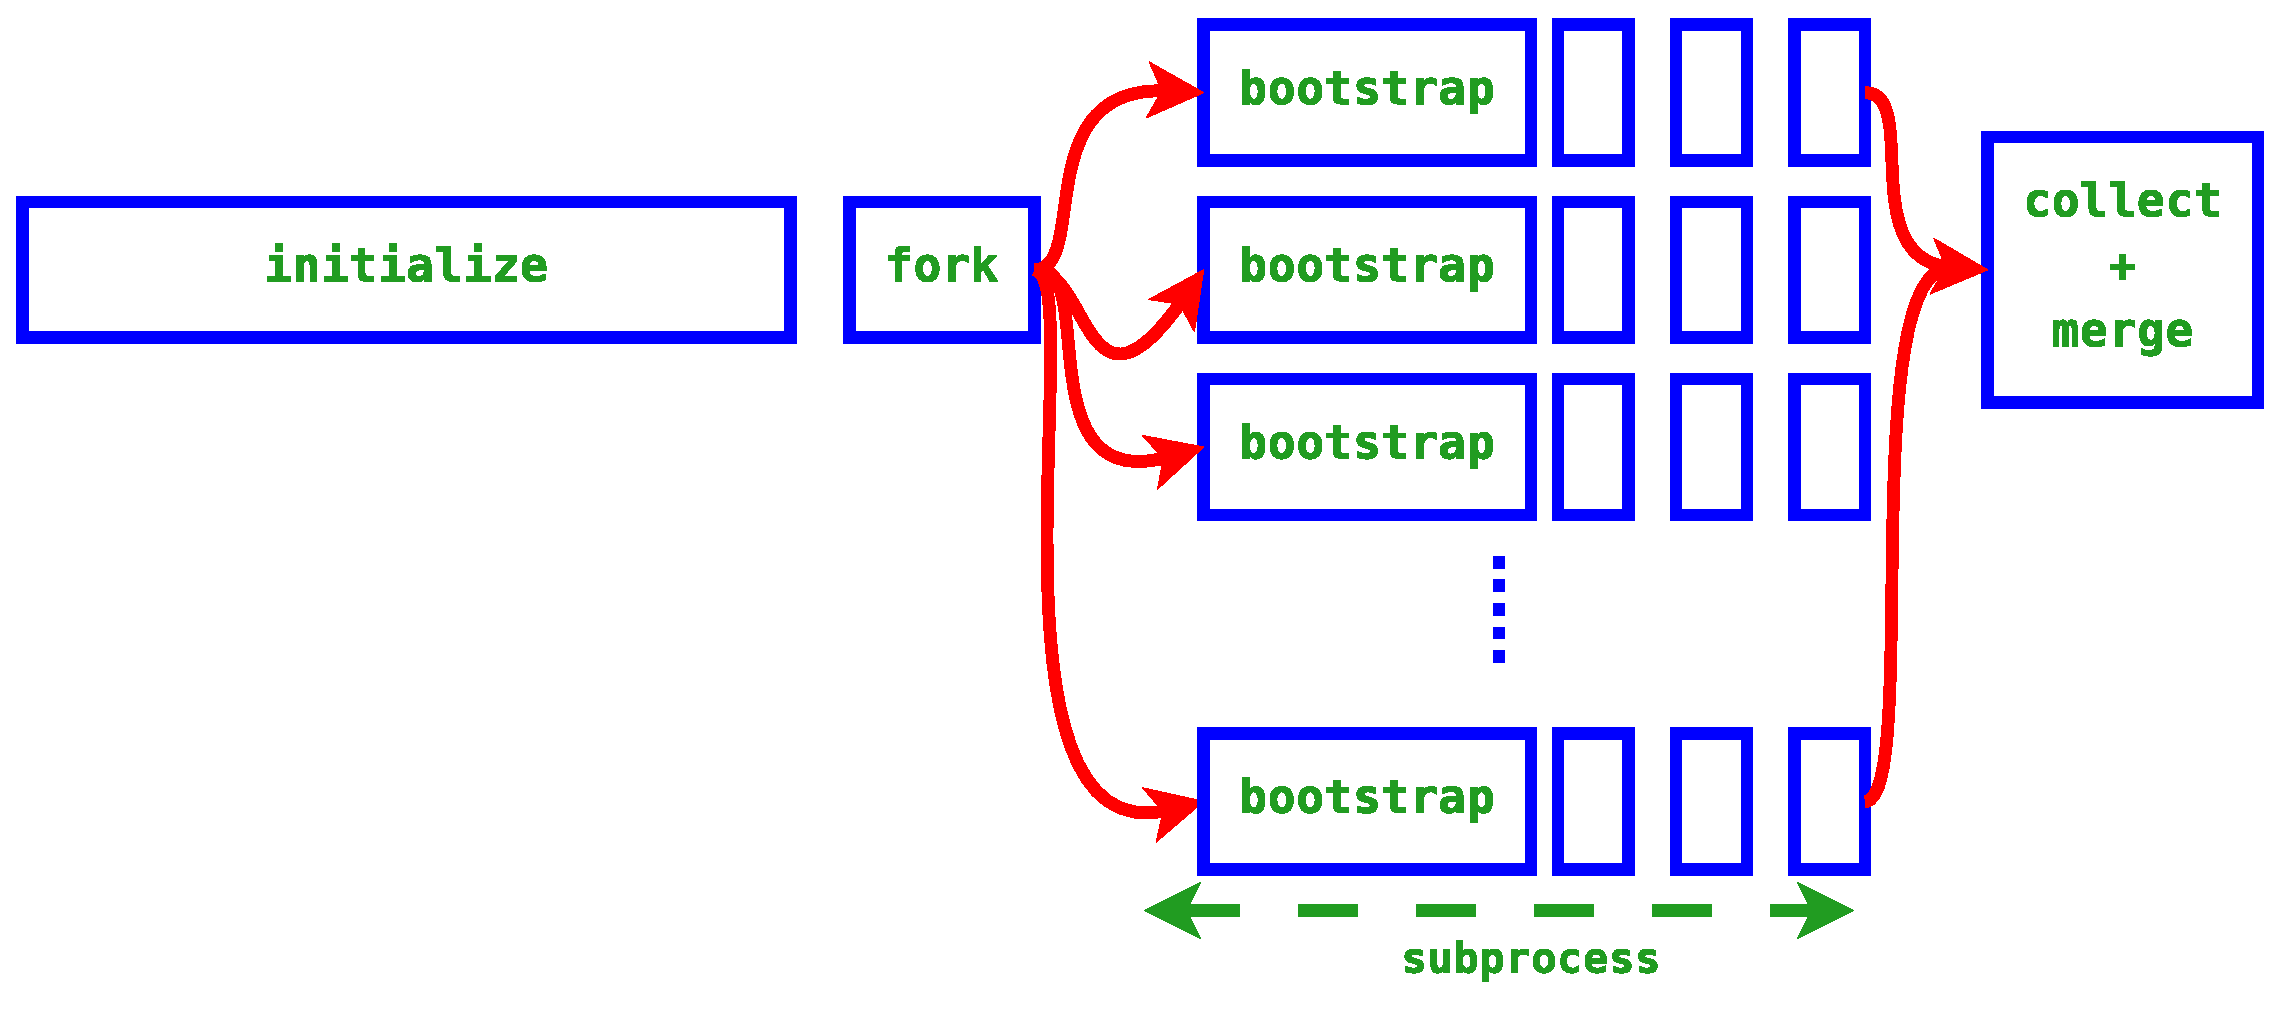
\includegraphics[angle=0,width=0.7\textwidth]{figs/athenamp-sequence.eps}
  \end{center}
\end{figure}
}

\begin{frame}[fragile]{}
%%   \begin{columns}
%%     \begin{column}{0.95\textwidth}

\begin{python}
class MpEventLoopMgr (PyAthena.Svc):
    def executeRun (self, maxevt):
        """Process `maxevt` events as Run (beginRun->endRun)"""
        if self._ncpus <= 0:
            return self._evtloop_mgr.executeRun(maxevt)

        import multiprocessing as mp
        info ("nbr of workers: %i", self._ncpus)
        info ("master workdir: %s", self._wkdir)
        wrks = mp.Pool(processes=self._ncpus,
                       initializer=self._worker_bootstrap)
        results = wrks.map_async(func=batch_run,
                                 iterable=(maxevt,)*self._ncpus)
\end{python}

\begin{exampleblock}{\bf{\myred{\texttt{\_worker\_bootstrap}}}}
\begin{itemize}
  \item function called after \texttt{fork}
  \item change work dir
  \item reopen file descriptors
  \item tickle the \texttt{IoComponentMgr}
\end{itemize}
\end{exampleblock}
%%     \end{column}
%%   \end{columns}
\end{frame}

\begin{frame}[fragile]{}

%%   \begin{columns}
%%     \begin{column}{0.95\textwidth}

\begin{python}
class MpEventLoopMgr (PyAthena.Svc):
    def executeRun (self, maxevt):
        """Process `maxevt` events as Run (beginRun->endRun)"""
        if self._ncpus <= 0:
            return self._evtloop_mgr.executeRun(maxevt)

        import multiprocessing as mp
        info ("nbr of workers: %i", self._ncpus)
        info ("master workdir: %s", self._wkdir)
        wrks = mp.Pool(processes=self._ncpus,
                       initializer=self._worker_bootstrap)
        results = wrks.map_async(func=batch_run,
                                 iterable=(maxevt,)*self._ncpus)
\end{python}

\begin{exampleblock}{\bf{\myred{\texttt{batch\_run}}}}
\begin{itemize}
  \item inject a filter algorithm in front of alg-sequence
    \begin{itemize}
      \item accept/reject events based on local process-id and current event number
    \end{itemize}
  \item effectively implement a round-robin filter
  \item call the \myred{\texttt{executeRun}} of the wrapped event loop manager
\end{itemize}
\end{exampleblock}
%%     \end{column}
%%   \end{columns}
\end{frame}

\begin{frame}[fragile]{}

  \begin{columns}
    \begin{column}{0.95\textwidth}

\begin{python}
class MpEventLoopMgr (PyAthena.Svc):
    def finalize (self): ...
\end{python}

\begin{block}{}
\begin{itemize}
  \item tickle \myred{\texttt{IIoComponentMgr::io\_finalize}} (when a forked process)
  \item master will run the merge of output files
    \begin{itemize}
      \item usually trivial for ROOT files containing histos and ntuples
      \item trickier for ROOT/POOL files
        \begin{itemize}
          \item have to take care of POOL links/references
        \end{itemize}
    \end{itemize}
\end{itemize}
\end{block}
    \end{column}
  \end{columns}
\end{frame}

\frame{
  \frametitle{Experiences with multi-processes}
\begin{block}{}
  \begin{itemize}
    \item limited long range impact
    \item modifications applied to control framework and I/O-related components
    \item easier to develop with
      \begin{itemize}
        \item no implicit sharing
        \item no lock, races, \ldots
      \end{itemize}
  \end{itemize}
\end{block}

\begin{alertblock}{Problems}
  \begin{itemize}
    \item random numbers, seeds and reproducibility
    \item I/O
      \begin{itemize}
        \item need to chase people directly \texttt{open()}ing files, by-passing framework hooks
        \item merging output files is tedious (but needed for production)
      \end{itemize}
    \item GRID
      \begin{itemize}
        \item submission of MP-jobs (overbooking computing nodes)
        \item \texttt{vmem} accounting
          \begin{itemize}
            \item most of grid resource monitoring tools will double-count the memory shared by \texttt{fork()}ed subprocesses
          \end{itemize}
      \end{itemize}
  \end{itemize}
\end{alertblock}
}

%%%%%%%%%%%%%%%%%%%%%%%%%%%%%%%%%%%%%%%%%%%%%%%%%%%%%%%%%%%%%%%%%%%%%%%%%%%%%%%
\section[Conclusions]{Conclusions}
\frame{
  \frametitle{Conclusions}

  \begin{block}{}
    \begin{itemize}
      \item experimented w/ both canonical ways of improving parallelism
        \begin{itemize}
          \item \myred{multi-threading: \texttt{AthenaMT}}
          \item \myred{multi-processes: \texttt{AthenaMP}}
        \end{itemize}
      \item multi-processes seem the less error-prone option while minimizing impact on clients' code
        \begin{itemize}
          \item note that \texttt{fork()+COW} may not be the \mypurple{only} way to achieve MP-parallelism with efficient (memory) resources sharing
        \end{itemize}
    \end{itemize}
  \end{block}

  \begin{exampleblock}{Prospects: MP+KSM}
    \begin{itemize}
      \item one fundamental flaw in \texttt{fork()+COW}:
        \begin{itemize}
          \item unshared memory can not be \mypurple{re-shared}
        \end{itemize}
      \item using a \emph{KSM}-enabled linux kernel, that flaw could be completely side-stepped
        \begin{itemize}
          \item see \emph{V. Innocente}'s talk on Thursday
        \end{itemize}
    \end{itemize}
  \end{exampleblock}
}

%%%%%%%%%%%%%%%%%%%%%%%%%%%%%%%%%%%%%%%%%%%%%%%%%%%%%%%%%%%%%%%%%%%%%%%%%%%%%%%
\frame{
  \begin{columns}
    \begin{column}{0.8\textwidth}
      \begin{block}{}
        \begin{center}
          Backup
        \end{center}
      \end{block}
    \end{column}
  \end{columns}
}

\frame{
%%   \frametitle{preliminary results}

%%   \begin{columns}
%%     \begin{column}{0.95\textwidth}

      \begin{exampleblock}{cpu}
        \texttt{4procs  242.85s user 8.71s system 249\% cpu 1:40.99 total}\\
        \texttt{3procs  213.67s user 7.30s system 191\% cpu 1:55.12 total}\\
        \texttt{2procs  181.67s user 6.13s system 149\% cpu 2:05.77 total}\\
        \texttt{1procs  162.52s user 5.22s system 093\% cpu 2:59.18 total}\\
        \texttt{0procs  160.25s user 4.28s system 094\% cpu 2:53.45 total}\\
      \end{exampleblock}
%%     \end{column}
%%   \end{columns}

 \begin{figure}
    \begin{center}
      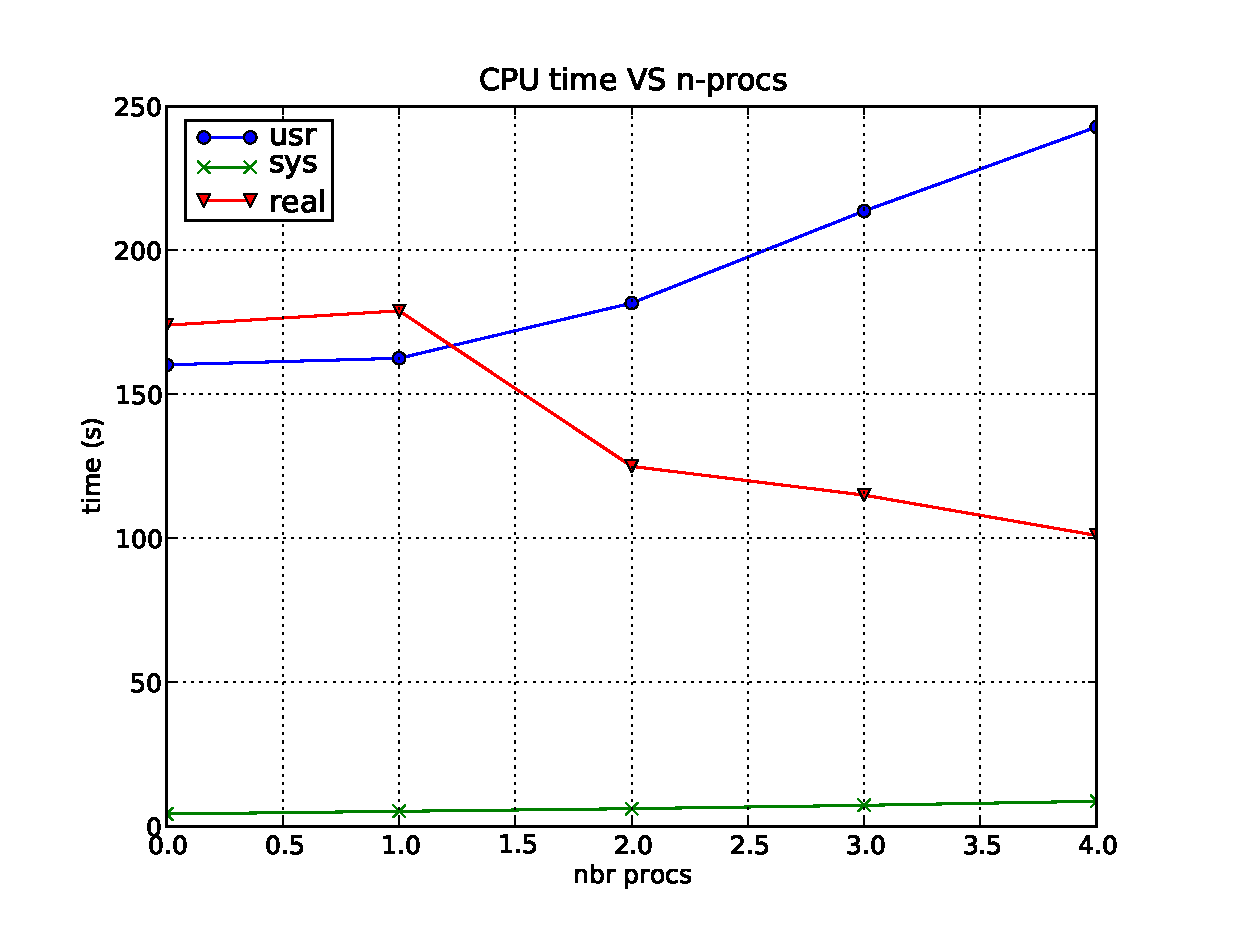
\includegraphics[angle=0,width=0.6\textwidth]{figs/cpu.eps}
    \end{center}
  \end{figure}
}

\frame{
%%   \frametitle{preliminary results - II}

%%   \begin{columns}
%%     \begin{column}{0.95\textwidth}

      \begin{exampleblock}{memory}
        process: $\sim 700MB\ VMem$ and $\sim 420MB\ RSS$\\
        \texttt{(before) evt 0: private: 004 MB | shared: 310 MB}\\
        \texttt{(before) evt 1: private: 235 MB | shared: 265 MB}\\
        \ldots\\
        \texttt{(before) evt50: private: 250 MB | shared: 263 MB}
      \end{exampleblock}
%%     \end{column}
%%   \end{columns}

 \begin{figure}
    \begin{center}
      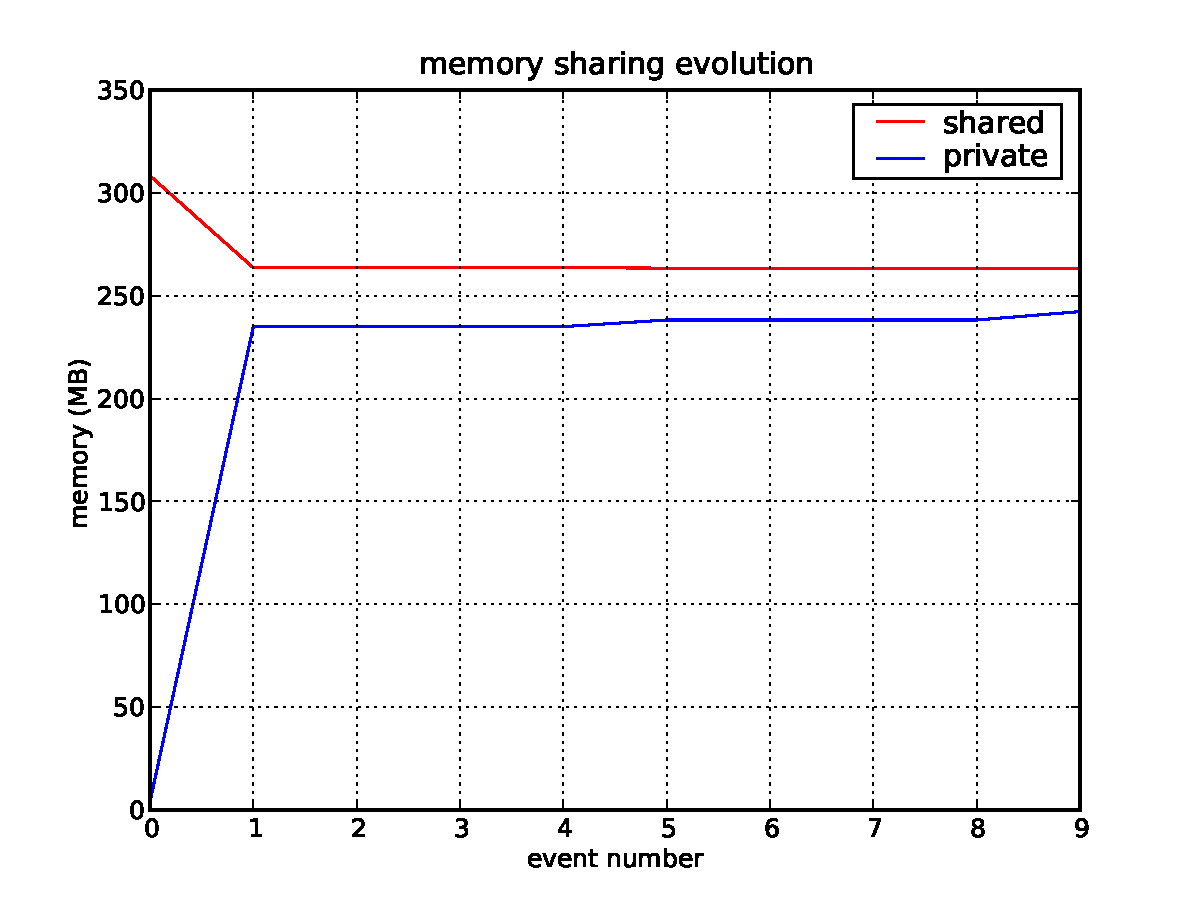
\includegraphics[angle=0,width=0.6\textwidth]{figs/data.epsi}
    \end{center}
  \end{figure}
}

\end{document}


